\documentclass{standalone}
\usepackage{tikz}
\usetikzlibrary{patterns, positioning}
\usepackage[sfdefault]{ClearSans} %% option 'sfdefault' activates Clear Sans as the default text font
\usepackage[T1]{fontenc}

\begin{document}
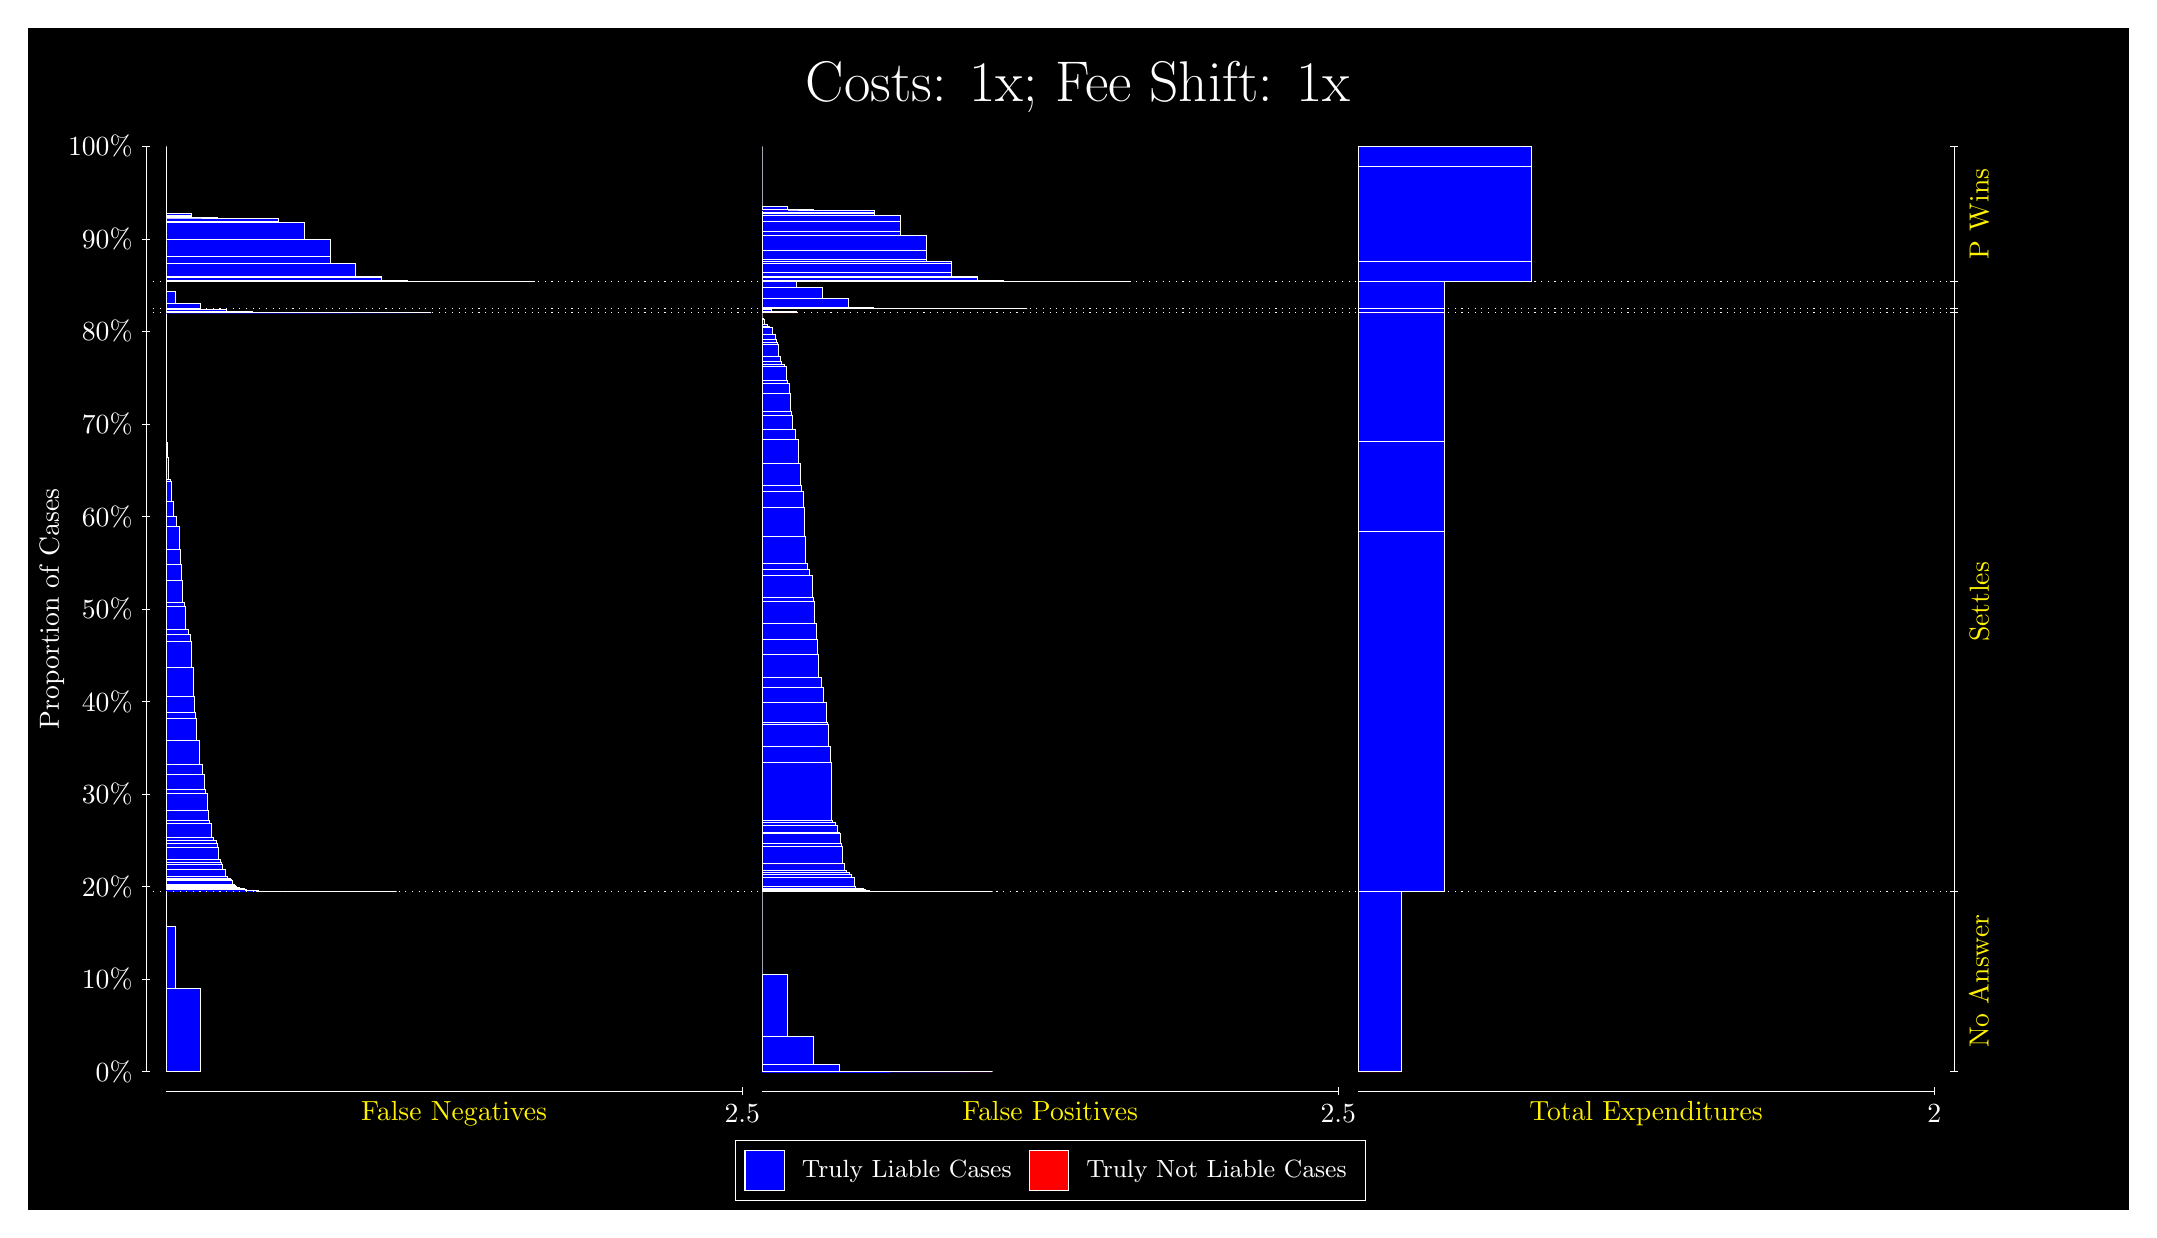
\begin{tikzpicture}
\draw[fill=black] (0,0) rectangle (26.667,15);
\draw[text=white] (0,13.5) rectangle (26.667,15) node[midway] {\huge Costs: 1x; Fee Shift: 1x};
\draw[white, very thin] (1.5,1.75) -- (1.5,13.5);
\node[rotate=90, text=white, anchor=center] at (0.3, 7.625) {Proportion of Cases};
\draw[white, very thin] (1.45,1.75) -- (1.55,1.75);
\node[text=white, anchor=east] at (1.45, 1.75) {0\%};
\draw[white, very thin] (1.45,2.925) -- (1.55,2.925);
\node[text=white, anchor=east] at (1.45, 2.925) {10\%};
\draw[white, very thin] (1.45,4.1) -- (1.55,4.1);
\node[text=white, anchor=east] at (1.45, 4.1) {20\%};
\draw[white, very thin] (1.45,5.275) -- (1.55,5.275);
\node[text=white, anchor=east] at (1.45, 5.275) {30\%};
\draw[white, very thin] (1.45,6.45) -- (1.55,6.45);
\node[text=white, anchor=east] at (1.45, 6.45) {40\%};
\draw[white, very thin] (1.45,7.625) -- (1.55,7.625);
\node[text=white, anchor=east] at (1.45, 7.625) {50\%};
\draw[white, very thin] (1.45,8.8) -- (1.55,8.8);
\node[text=white, anchor=east] at (1.45, 8.8) {60\%};
\draw[white, very thin] (1.45,9.975) -- (1.55,9.975);
\node[text=white, anchor=east] at (1.45, 9.975) {70\%};
\draw[white, very thin] (1.45,11.15) -- (1.55,11.15);
\node[text=white, anchor=east] at (1.45, 11.15) {80\%};
\draw[white, very thin] (1.45,12.325) -- (1.55,12.325);
\node[text=white, anchor=east] at (1.45, 12.325) {90\%};
\draw[white, very thin] (1.45,13.5) -- (1.55,13.5);
\node[text=white, anchor=east] at (1.45, 13.5) {100\%};

\draw[white, very thin] (24.457,1.75) -- (24.457,13.5);
\draw[white, very thin] (24.407,1.75) -- (24.507,1.75);
\node[anchor=west] at (24.407, 1.75) {};
\draw[white, very thin] (24.407,4.0413) -- (24.507,4.0413);
\node[anchor=west] at (24.407, 4.0413) {};
\draw[white, very thin] (24.407,11.388) -- (24.507,11.388);
\node[anchor=west] at (24.407, 11.388) {};
\draw[white, very thin] (24.407,11.442) -- (24.507,11.442);
\node[anchor=west] at (24.407, 11.442) {};
\draw[white, very thin] (24.407,11.784) -- (24.507,11.784);
\node[anchor=west] at (24.407, 11.784) {};
\draw[white, very thin] (24.407,13.5) -- (24.507,13.5);
\node[anchor=west] at (24.407, 13.5) {};

\draw[white, very thin, fill=blue] (1.75,1.75) rectangle (2.1891,2.8115);
\draw[white, very thin, fill=blue] (1.75,2.8115) rectangle (1.8638,3.598);
\draw[white, very thin, fill=red] (1.75,3.598) rectangle (1.75,3.598);
\draw[white, very thin, fill=blue] (1.75,3.598) rectangle (1.75,4.0413);
\draw[white, very thin, fill=blue] (1.75,4.0413) rectangle (4.6775,4.0413);
\draw[white, very thin, fill=blue] (1.75,4.0413) rectangle (4.5312,4.0413);
\draw[white, very thin, fill=blue] (1.75,4.0413) rectangle (4.3848,4.0413);
\draw[white, very thin, fill=blue] (1.75,4.0413) rectangle (4.3523,4.0413);
\draw[white, very thin, fill=blue] (1.75,4.0413) rectangle (4.2384,4.0413);
\draw[white, very thin, fill=blue] (1.75,4.0413) rectangle (4.2059,4.0413);
\draw[white, very thin, fill=blue] (1.75,4.0413) rectangle (4.092,4.0413);
\draw[white, very thin, fill=blue] (1.75,4.0413) rectangle (4.0595,4.0413);
\draw[white, very thin, fill=blue] (1.75,4.0413) rectangle (4.027,4.0413);
\draw[white, very thin, fill=blue] (1.75,4.0413) rectangle (3.9457,4.0413);
\draw[white, very thin, fill=blue] (1.75,4.0413) rectangle (3.9131,4.0413);
\draw[white, very thin, fill=blue] (1.75,4.0413) rectangle (3.8806,4.0413);
\draw[white, very thin, fill=blue] (1.75,4.0413) rectangle (3.7993,4.0413);
\draw[white, very thin, fill=blue] (1.75,4.0413) rectangle (3.7668,4.0413);
\draw[white, very thin, fill=blue] (1.75,4.0413) rectangle (3.7342,4.0413);
\draw[white, very thin, fill=blue] (1.75,4.0413) rectangle (3.7017,4.0413);
\draw[white, very thin, fill=blue] (1.75,4.0413) rectangle (3.6529,4.0413);
\draw[white, very thin, fill=blue] (1.75,4.0413) rectangle (3.6204,4.0413);
\draw[white, very thin, fill=blue] (1.75,4.0413) rectangle (3.5878,4.0413);
\draw[white, very thin, fill=blue] (1.75,4.0413) rectangle (3.5553,4.0413);
\draw[white, very thin, fill=blue] (1.75,4.0413) rectangle (3.5065,4.0413);
\draw[white, very thin, fill=blue] (1.75,4.0413) rectangle (3.474,4.0413);
\draw[white, very thin, fill=blue] (1.75,4.0413) rectangle (3.4415,4.0413);
\draw[white, very thin, fill=blue] (1.75,4.0413) rectangle (3.4089,4.0413);
\draw[white, very thin, fill=blue] (1.75,4.0413) rectangle (3.3764,4.0413);
\draw[white, very thin, fill=blue] (1.75,4.0413) rectangle (3.3602,4.0413);
\draw[white, very thin, fill=blue] (1.75,4.0413) rectangle (3.3276,4.0413);
\draw[white, very thin, fill=blue] (1.75,4.0413) rectangle (3.2951,4.0413);
\draw[white, very thin, fill=blue] (1.75,4.0413) rectangle (3.2626,4.0413);
\draw[white, very thin, fill=blue] (1.75,4.0413) rectangle (3.23,4.0413);
\draw[white, very thin, fill=blue] (1.75,4.0413) rectangle (3.2138,4.0413);
\draw[white, very thin, fill=blue] (1.75,4.0413) rectangle (3.1812,4.0413);
\draw[white, very thin, fill=blue] (1.75,4.0413) rectangle (3.1487,4.0414);
\draw[white, very thin, fill=blue] (1.75,4.0414) rectangle (3.1162,4.0414);
\draw[white, very thin, fill=blue] (1.75,4.0414) rectangle (3.0837,4.0414);
\draw[white, very thin, fill=blue] (1.75,4.0414) rectangle (3.0674,4.0419);
\draw[white, very thin, fill=blue] (1.75,4.0419) rectangle (3.0511,4.042);
\draw[white, very thin, fill=blue] (1.75,4.042) rectangle (3.0349,4.042);
\draw[white, very thin, fill=blue] (1.75,4.042) rectangle (3.0023,4.042);
\draw[white, very thin, fill=blue] (1.75,4.042) rectangle (2.9698,4.0425);
\draw[white, very thin, fill=blue] (1.75,4.0425) rectangle (2.9373,4.0426);
\draw[white, very thin, fill=blue] (1.75,4.0426) rectangle (2.921,4.0474);
\draw[white, very thin, fill=blue] (1.75,4.0474) rectangle (2.9048,4.0474);
\draw[white, very thin, fill=blue] (1.75,4.0474) rectangle (2.8885,4.048);
\draw[white, very thin, fill=blue] (1.75,4.048) rectangle (2.856,4.0485);
\draw[white, very thin, fill=blue] (1.75,4.0485) rectangle (2.8234,4.0533);
\draw[white, very thin, fill=blue] (1.75,4.0533) rectangle (2.7909,4.0559);
\draw[white, very thin, fill=blue] (1.75,4.0559) rectangle (2.7746,4.0596);
\draw[white, very thin, fill=blue] (1.75,4.0596) rectangle (2.7584,4.0602);
\draw[white, very thin, fill=blue] (1.75,4.0602) rectangle (2.7421,4.0764);
\draw[white, very thin, fill=blue] (1.75,4.0764) rectangle (2.7258,4.0789);
\draw[white, very thin, fill=blue] (1.75,4.0789) rectangle (2.7096,4.082);
\draw[white, very thin, fill=blue] (1.75,4.082) rectangle (2.6771,4.0838);
\draw[white, very thin, fill=blue] (1.75,4.0838) rectangle (2.6445,4.1055);
\draw[white, very thin, fill=blue] (1.75,4.1055) rectangle (2.6283,4.1169);
\draw[white, very thin, fill=blue] (1.75,4.1169) rectangle (2.612,4.1258);
\draw[white, very thin, fill=blue] (1.75,4.1258) rectangle (2.5957,4.1839);
\draw[white, very thin, fill=blue] (1.75,4.1839) rectangle (2.5795,4.1867);
\draw[white, very thin, fill=blue] (1.75,4.1867) rectangle (2.5632,4.2099);
\draw[white, very thin, fill=blue] (1.75,4.2099) rectangle (2.5307,4.2307);
\draw[white, very thin, fill=blue] (1.75,4.2307) rectangle (2.4982,4.3193);
\draw[white, very thin, fill=blue] (1.75,4.3193) rectangle (2.4656,4.381);
\draw[white, very thin, fill=blue] (1.75,4.381) rectangle (2.4494,4.413);
\draw[white, very thin, fill=blue] (1.75,4.413) rectangle (2.4331,4.4419);
\draw[white, very thin, fill=blue] (1.75,4.4419) rectangle (2.4168,4.597);
\draw[white, very thin, fill=blue] (1.75,4.597) rectangle (2.4006,4.6551);
\draw[white, very thin, fill=blue] (1.75,4.6551) rectangle (2.3843,4.6918);
\draw[white, very thin, fill=blue] (1.75,4.6918) rectangle (2.3518,4.7209);
\draw[white, very thin, fill=blue] (1.75,4.7209) rectangle (2.3192,4.9001);
\draw[white, very thin, fill=blue] (1.75,4.9001) rectangle (2.303,4.9448);
\draw[white, very thin, fill=blue] (1.75,4.9448) rectangle (2.2867,5.0623);
\draw[white, very thin, fill=blue] (1.75,5.0623) rectangle (2.2705,5.2896);
\draw[white, very thin, fill=blue] (1.75,5.2896) rectangle (2.2542,5.3402);
\draw[white, very thin, fill=blue] (1.75,5.3402) rectangle (2.2379,5.5264);
\draw[white, very thin, fill=blue] (1.75,5.5264) rectangle (2.2054,5.6547);
\draw[white, very thin, fill=blue] (1.75,5.6547) rectangle (2.1729,5.9534);
\draw[white, very thin, fill=blue] (1.75,5.9534) rectangle (2.1403,6.2398);
\draw[white, very thin, fill=blue] (1.75,6.2398) rectangle (2.1241,6.3105);
\draw[white, very thin, fill=blue] (1.75,6.3105) rectangle (2.1078,6.5124);
\draw[white, very thin, fill=blue] (1.75,6.5124) rectangle (2.0915,6.8813);
\draw[white, very thin, fill=blue] (1.75,6.8813) rectangle (2.0753,7.22);
\draw[white, very thin, fill=blue] (1.75,7.22) rectangle (2.059,7.2993);
\draw[white, very thin, fill=blue] (1.75,7.2993) rectangle (2.0265,7.3725);
\draw[white, very thin, fill=blue] (1.75,7.3725) rectangle (1.994,7.6585);
\draw[white, very thin, fill=blue] (1.75,7.6585) rectangle (1.9777,7.7083);
\draw[white, very thin, fill=blue] (1.75,7.7083) rectangle (1.9614,7.9915);
\draw[white, very thin, fill=blue] (1.75,7.9915) rectangle (1.9452,8.1958);
\draw[white, very thin, fill=blue] (1.75,8.1958) rectangle (1.9289,8.3836);
\draw[white, very thin, fill=blue] (1.75,8.3836) rectangle (1.9126,8.6734);
\draw[white, very thin, fill=blue] (1.75,8.6734) rectangle (1.8801,8.8004);
\draw[white, very thin, fill=blue] (1.75,8.8004) rectangle (1.8476,8.9956);
\draw[white, very thin, fill=blue] (1.75,8.9956) rectangle (1.8151,9.2435);
\draw[white, very thin, fill=blue] (1.75,9.2435) rectangle (1.7988,9.2713);
\draw[white, very thin, fill=blue] (1.75,9.2713) rectangle (1.7825,9.5478);
\draw[white, very thin, fill=blue] (1.75,9.5478) rectangle (1.7663,9.7472);
\draw[white, very thin, fill=red] (1.75,9.7472) rectangle (1.75,9.7472);
\draw[white, very thin, fill=blue] (1.75,9.7472) rectangle (1.75,11.388);
\draw[white, very thin, fill=blue] (1.75,11.388) rectangle (5.1167,11.388);
\draw[white, very thin, fill=blue] (1.75,11.388) rectangle (4.7914,11.388);
\draw[white, very thin, fill=blue] (1.75,11.388) rectangle (4.4661,11.388);
\draw[white, very thin, fill=blue] (1.75,11.388) rectangle (4.1408,11.388);
\draw[white, very thin, fill=blue] (1.75,11.388) rectangle (3.8155,11.388);
\draw[white, very thin, fill=blue] (1.75,11.388) rectangle (3.4903,11.388);
\draw[white, very thin, fill=blue] (1.75,11.388) rectangle (3.165,11.39);
\draw[white, very thin, fill=blue] (1.75,11.39) rectangle (2.8397,11.404);
\draw[white, very thin, fill=blue] (1.75,11.404) rectangle (2.5144,11.428);
\draw[white, very thin, fill=blue] (1.75,11.428) rectangle (2.1891,11.442);
\draw[white, very thin, fill=red] (1.75,11.442) rectangle (1.75,11.442);
\draw[white, very thin, fill=blue] (1.75,11.442) rectangle (2.1891,11.51);
\draw[white, very thin, fill=blue] (1.75,11.51) rectangle (1.8638,11.657);
\draw[white, very thin, fill=red] (1.75,11.657) rectangle (1.75,11.657);
\draw[white, very thin, fill=blue] (1.75,11.657) rectangle (1.75,11.784);
\draw[white, very thin, fill=blue] (1.75,11.784) rectangle (6.4341,11.784);
\draw[white, very thin, fill=blue] (1.75,11.784) rectangle (6.1088,11.784);
\draw[white, very thin, fill=blue] (1.75,11.784) rectangle (5.7835,11.784);
\draw[white, very thin, fill=blue] (1.75,11.784) rectangle (5.4582,11.784);
\draw[white, very thin, fill=blue] (1.75,11.784) rectangle (5.1329,11.785);
\draw[white, very thin, fill=blue] (1.75,11.785) rectangle (4.8077,11.789);
\draw[white, very thin, fill=blue] (1.75,11.789) rectangle (4.8077,11.794);
\draw[white, very thin, fill=blue] (1.75,11.794) rectangle (4.4824,11.84);
\draw[white, very thin, fill=blue] (1.75,11.84) rectangle (4.4824,11.844);
\draw[white, very thin, fill=blue] (1.75,11.844) rectangle (4.1571,12.011);
\draw[white, very thin, fill=blue] (1.75,12.011) rectangle (4.027,12.011);
\draw[white, very thin, fill=blue] (1.75,12.011) rectangle (3.8318,12.098);
\draw[white, very thin, fill=blue] (1.75,12.098) rectangle (3.8318,12.315);
\draw[white, very thin, fill=blue] (1.75,12.315) rectangle (3.7017,12.315);
\draw[white, very thin, fill=blue] (1.75,12.315) rectangle (3.7017,12.315);
\draw[white, very thin, fill=blue] (1.75,12.315) rectangle (3.5065,12.541);
\draw[white, very thin, fill=blue] (1.75,12.541) rectangle (3.3764,12.541);
\draw[white, very thin, fill=blue] (1.75,12.541) rectangle (3.1812,12.542);
\draw[white, very thin, fill=blue] (1.75,12.542) rectangle (3.1812,12.588);
\draw[white, very thin, fill=blue] (1.75,12.588) rectangle (3.1812,12.589);
\draw[white, very thin, fill=blue] (1.75,12.589) rectangle (3.0511,12.589);
\draw[white, very thin, fill=blue] (1.75,12.589) rectangle (3.0511,12.589);
\draw[white, very thin, fill=blue] (1.75,12.589) rectangle (2.856,12.59);
\draw[white, very thin, fill=blue] (1.75,12.59) rectangle (2.856,12.59);
\draw[white, very thin, fill=blue] (1.75,12.59) rectangle (2.7258,12.59);
\draw[white, very thin, fill=blue] (1.75,12.59) rectangle (2.7258,12.59);
\draw[white, very thin, fill=blue] (1.75,12.59) rectangle (2.7258,12.59);
\draw[white, very thin, fill=blue] (1.75,12.59) rectangle (2.5307,12.59);
\draw[white, very thin, fill=blue] (1.75,12.59) rectangle (2.5307,12.59);
\draw[white, very thin, fill=blue] (1.75,12.59) rectangle (2.4006,12.59);
\draw[white, very thin, fill=blue] (1.75,12.59) rectangle (2.4006,12.594);
\draw[white, very thin, fill=blue] (1.75,12.594) rectangle (2.2054,12.594);
\draw[white, very thin, fill=blue] (1.75,12.594) rectangle (2.2054,12.594);
\draw[white, very thin, fill=blue] (1.75,12.594) rectangle (2.0753,12.616);
\draw[white, very thin, fill=blue] (1.75,12.616) rectangle (2.0753,12.624);
\draw[white, very thin, fill=blue] (1.75,12.624) rectangle (2.0753,12.655);
\draw[white, very thin, fill=blue] (1.75,12.655) rectangle (1.8801,12.655);
\draw[white, very thin, fill=blue] (1.75,12.655) rectangle (1.8801,12.655);
\draw[white, very thin, fill=red] (1.75,12.655) rectangle (1.75,12.655);
\draw[white, very thin, fill=blue] (1.75,12.655) rectangle (1.75,13.5);
\draw[white, very thin, fill=red] (9.3189,1.75) rectangle (12.246,1.75);
\draw[white, very thin, fill=blue] (9.3189,1.75) rectangle (12.246,1.75);
\draw[white, very thin, fill=blue] (9.3189,1.75) rectangle (11.921,1.75);
\draw[white, very thin, fill=blue] (9.3189,1.75) rectangle (11.596,1.75);
\draw[white, very thin, fill=blue] (9.3189,1.75) rectangle (11.271,1.75);
\draw[white, very thin, fill=blue] (9.3189,1.75) rectangle (10.945,1.7503);
\draw[white, very thin, fill=blue] (9.3189,1.7503) rectangle (10.62,1.7576);
\draw[white, very thin, fill=blue] (9.3189,1.7576) rectangle (10.295,1.8358);
\draw[white, very thin, fill=blue] (9.3189,1.8358) rectangle (9.9694,2.1933);
\draw[white, very thin, fill=blue] (9.3189,2.1933) rectangle (9.6442,2.9798);
\draw[white, very thin, fill=blue] (9.3189,2.9798) rectangle (9.3189,4.0413);
\draw[white, very thin, fill=red] (9.3189,4.0413) rectangle (12.246,4.0413);
\draw[white, very thin, fill=blue] (9.3189,4.0413) rectangle (12.246,4.0413);
\draw[white, very thin, fill=red] (9.3189,4.0413) rectangle (12.1,4.0413);
\draw[white, very thin, fill=blue] (9.3189,4.0413) rectangle (12.1,4.0413);
\draw[white, very thin, fill=red] (9.3189,4.0413) rectangle (11.954,4.0413);
\draw[white, very thin, fill=blue] (9.3189,4.0413) rectangle (11.954,4.0413);
\draw[white, very thin, fill=blue] (9.3189,4.0413) rectangle (11.921,4.0413);
\draw[white, very thin, fill=red] (9.3189,4.0413) rectangle (11.807,4.0413);
\draw[white, very thin, fill=blue] (9.3189,4.0413) rectangle (11.807,4.0413);
\draw[white, very thin, fill=blue] (9.3189,4.0413) rectangle (11.775,4.0413);
\draw[white, very thin, fill=red] (9.3189,4.0413) rectangle (11.661,4.0413);
\draw[white, very thin, fill=blue] (9.3189,4.0413) rectangle (11.661,4.0413);
\draw[white, very thin, fill=blue] (9.3189,4.0413) rectangle (11.628,4.0413);
\draw[white, very thin, fill=blue] (9.3189,4.0413) rectangle (11.596,4.0413);
\draw[white, very thin, fill=red] (9.3189,4.0413) rectangle (11.515,4.0413);
\draw[white, very thin, fill=blue] (9.3189,4.0413) rectangle (11.515,4.0413);
\draw[white, very thin, fill=blue] (9.3189,4.0413) rectangle (11.482,4.0413);
\draw[white, very thin, fill=blue] (9.3189,4.0413) rectangle (11.449,4.0413);
\draw[white, very thin, fill=red] (9.3189,4.0413) rectangle (11.368,4.0413);
\draw[white, very thin, fill=blue] (9.3189,4.0413) rectangle (11.368,4.0413);
\draw[white, very thin, fill=blue] (9.3189,4.0413) rectangle (11.336,4.0413);
\draw[white, very thin, fill=blue] (9.3189,4.0413) rectangle (11.303,4.0413);
\draw[white, very thin, fill=blue] (9.3189,4.0413) rectangle (11.271,4.0413);
\draw[white, very thin, fill=red] (9.3189,4.0413) rectangle (11.222,4.0413);
\draw[white, very thin, fill=blue] (9.3189,4.0413) rectangle (11.222,4.0413);
\draw[white, very thin, fill=blue] (9.3189,4.0413) rectangle (11.189,4.0413);
\draw[white, very thin, fill=blue] (9.3189,4.0413) rectangle (11.157,4.0413);
\draw[white, very thin, fill=blue] (9.3189,4.0413) rectangle (11.124,4.0413);
\draw[white, very thin, fill=red] (9.3189,4.0413) rectangle (11.075,4.0413);
\draw[white, very thin, fill=blue] (9.3189,4.0413) rectangle (11.075,4.0413);
\draw[white, very thin, fill=blue] (9.3189,4.0413) rectangle (11.043,4.0413);
\draw[white, very thin, fill=blue] (9.3189,4.0413) rectangle (11.01,4.0414);
\draw[white, very thin, fill=blue] (9.3189,4.0414) rectangle (10.978,4.0414);
\draw[white, very thin, fill=blue] (9.3189,4.0414) rectangle (10.945,4.0414);
\draw[white, very thin, fill=red] (9.3189,4.0414) rectangle (10.929,4.0414);
\draw[white, very thin, fill=blue] (9.3189,4.0414) rectangle (10.929,4.0415);
\draw[white, very thin, fill=blue] (9.3189,4.0415) rectangle (10.896,4.0415);
\draw[white, very thin, fill=blue] (9.3189,4.0415) rectangle (10.864,4.0415);
\draw[white, very thin, fill=blue] (9.3189,4.0415) rectangle (10.831,4.042);
\draw[white, very thin, fill=blue] (9.3189,4.042) rectangle (10.799,4.042);
\draw[white, very thin, fill=red] (9.3189,4.042) rectangle (10.783,4.042);
\draw[white, very thin, fill=blue] (9.3189,4.042) rectangle (10.783,4.0438);
\draw[white, very thin, fill=blue] (9.3189,4.0438) rectangle (10.75,4.0444);
\draw[white, very thin, fill=blue] (9.3189,4.0444) rectangle (10.718,4.0449);
\draw[white, very thin, fill=blue] (9.3189,4.0449) rectangle (10.685,4.0497);
\draw[white, very thin, fill=blue] (9.3189,4.0497) rectangle (10.653,4.0511);
\draw[white, very thin, fill=red] (9.3189,4.0511) rectangle (10.636,4.0511);
\draw[white, very thin, fill=blue] (9.3189,4.0511) rectangle (10.636,4.0697);
\draw[white, very thin, fill=blue] (9.3189,4.0697) rectangle (10.62,4.0702);
\draw[white, very thin, fill=blue] (9.3189,4.0702) rectangle (10.604,4.0759);
\draw[white, very thin, fill=blue] (9.3189,4.0759) rectangle (10.571,4.0777);
\draw[white, very thin, fill=blue] (9.3189,4.0777) rectangle (10.539,4.0795);
\draw[white, very thin, fill=blue] (9.3189,4.0795) rectangle (10.506,4.1021);
\draw[white, very thin, fill=red] (9.3189,4.1021) rectangle (10.49,4.1021);
\draw[white, very thin, fill=blue] (9.3189,4.1021) rectangle (10.49,4.216);
\draw[white, very thin, fill=blue] (9.3189,4.216) rectangle (10.474,4.2178);
\draw[white, very thin, fill=blue] (9.3189,4.2178) rectangle (10.457,4.2593);
\draw[white, very thin, fill=blue] (9.3189,4.2593) rectangle (10.425,4.2839);
\draw[white, very thin, fill=blue] (9.3189,4.2839) rectangle (10.392,4.3039);
\draw[white, very thin, fill=blue] (9.3189,4.3039) rectangle (10.36,4.3911);
\draw[white, very thin, fill=red] (9.3189,4.3911) rectangle (10.344,4.3911);
\draw[white, very thin, fill=blue] (9.3189,4.3911) rectangle (10.344,4.607);
\draw[white, very thin, fill=blue] (9.3189,4.607) rectangle (10.327,4.645);
\draw[white, very thin, fill=blue] (9.3189,4.645) rectangle (10.311,4.78);
\draw[white, very thin, fill=blue] (9.3189,4.78) rectangle (10.295,4.7919);
\draw[white, very thin, fill=blue] (9.3189,4.7919) rectangle (10.278,4.881);
\draw[white, very thin, fill=blue] (9.3189,4.881) rectangle (10.246,4.91);
\draw[white, very thin, fill=blue] (9.3189,4.91) rectangle (10.213,4.9395);
\draw[white, very thin, fill=red] (9.3189,4.9395) rectangle (10.197,4.9395);
\draw[white, very thin, fill=blue] (9.3189,4.9395) rectangle (10.197,5.6825);
\draw[white, very thin, fill=blue] (9.3189,5.6825) rectangle (10.181,5.8819);
\draw[white, very thin, fill=blue] (9.3189,5.8819) rectangle (10.165,6.1583);
\draw[white, very thin, fill=blue] (9.3189,6.1583) rectangle (10.148,6.1862);
\draw[white, very thin, fill=blue] (9.3189,6.1862) rectangle (10.132,6.434);
\draw[white, very thin, fill=blue] (9.3189,6.434) rectangle (10.1,6.6292);
\draw[white, very thin, fill=blue] (9.3189,6.6292) rectangle (10.067,6.7562);
\draw[white, very thin, fill=blue] (9.3189,6.7562) rectangle (10.034,7.046);
\draw[white, very thin, fill=blue] (9.3189,7.046) rectangle (10.018,7.2338);
\draw[white, very thin, fill=blue] (9.3189,7.2338) rectangle (10.002,7.4381);
\draw[white, very thin, fill=blue] (9.3189,7.4381) rectangle (9.9857,7.7213);
\draw[white, very thin, fill=blue] (9.3189,7.7213) rectangle (9.9694,7.7711);
\draw[white, very thin, fill=blue] (9.3189,7.7711) rectangle (9.9532,8.0571);
\draw[white, very thin, fill=blue] (9.3189,8.0571) rectangle (9.9206,8.1303);
\draw[white, very thin, fill=blue] (9.3189,8.1303) rectangle (9.8881,8.2096);
\draw[white, very thin, fill=blue] (9.3189,8.2096) rectangle (9.8718,8.5483);
\draw[white, very thin, fill=blue] (9.3189,8.5483) rectangle (9.8556,8.9173);
\draw[white, very thin, fill=blue] (9.3189,8.9173) rectangle (9.8393,9.1191);
\draw[white, very thin, fill=blue] (9.3189,9.1191) rectangle (9.8231,9.1899);
\draw[white, very thin, fill=blue] (9.3189,9.1899) rectangle (9.8068,9.4762);
\draw[white, very thin, fill=blue] (9.3189,9.4762) rectangle (9.7743,9.7749);
\draw[white, very thin, fill=blue] (9.3189,9.7749) rectangle (9.7417,9.9032);
\draw[white, very thin, fill=blue] (9.3189,9.9032) rectangle (9.7092,10.089);
\draw[white, very thin, fill=blue] (9.3189,10.089) rectangle (9.6929,10.14);
\draw[white, very thin, fill=blue] (9.3189,10.14) rectangle (9.6767,10.367);
\draw[white, very thin, fill=blue] (9.3189,10.367) rectangle (9.6604,10.485);
\draw[white, very thin, fill=blue] (9.3189,10.485) rectangle (9.6442,10.529);
\draw[white, very thin, fill=blue] (9.3189,10.529) rectangle (9.6279,10.709);
\draw[white, very thin, fill=blue] (9.3189,10.709) rectangle (9.5954,10.738);
\draw[white, very thin, fill=blue] (9.3189,10.738) rectangle (9.5628,10.775);
\draw[white, very thin, fill=blue] (9.3189,10.775) rectangle (9.5466,10.833);
\draw[white, very thin, fill=blue] (9.3189,10.833) rectangle (9.5303,10.988);
\draw[white, very thin, fill=blue] (9.3189,10.988) rectangle (9.514,11.017);
\draw[white, very thin, fill=blue] (9.3189,11.017) rectangle (9.4978,11.049);
\draw[white, very thin, fill=blue] (9.3189,11.049) rectangle (9.4815,11.11);
\draw[white, very thin, fill=blue] (9.3189,11.11) rectangle (9.449,11.199);
\draw[white, very thin, fill=blue] (9.3189,11.199) rectangle (9.4165,11.22);
\draw[white, very thin, fill=blue] (9.3189,11.22) rectangle (9.3839,11.243);
\draw[white, very thin, fill=blue] (9.3189,11.243) rectangle (9.3677,11.246);
\draw[white, very thin, fill=blue] (9.3189,11.246) rectangle (9.3514,11.304);
\draw[white, very thin, fill=blue] (9.3189,11.304) rectangle (9.3351,11.313);
\draw[white, very thin, fill=blue] (9.3189,11.313) rectangle (9.3189,11.388);
\draw[white, very thin, fill=red] (9.3189,11.388) rectangle (9.758,11.388);
\draw[white, very thin, fill=blue] (9.3189,11.388) rectangle (9.758,11.402);
\draw[white, very thin, fill=blue] (9.3189,11.402) rectangle (9.4327,11.426);
\draw[white, very thin, fill=blue] (9.3189,11.426) rectangle (9.3189,11.442);
\draw[white, very thin, fill=red] (9.3189,11.442) rectangle (12.686,11.442);
\draw[white, very thin, fill=blue] (9.3189,11.442) rectangle (12.686,11.442);
\draw[white, very thin, fill=blue] (9.3189,11.442) rectangle (12.36,11.442);
\draw[white, very thin, fill=blue] (9.3189,11.442) rectangle (12.035,11.442);
\draw[white, very thin, fill=blue] (9.3189,11.442) rectangle (11.71,11.442);
\draw[white, very thin, fill=blue] (9.3189,11.442) rectangle (11.384,11.442);
\draw[white, very thin, fill=blue] (9.3189,11.442) rectangle (11.059,11.443);
\draw[white, very thin, fill=blue] (9.3189,11.443) rectangle (10.734,11.461);
\draw[white, very thin, fill=blue] (9.3189,11.461) rectangle (10.409,11.568);
\draw[white, very thin, fill=blue] (9.3189,11.568) rectangle (10.083,11.715);
\draw[white, very thin, fill=blue] (9.3189,11.715) rectangle (9.758,11.784);
\draw[white, very thin, fill=red] (9.3189,11.784) rectangle (14.003,11.784);
\draw[white, very thin, fill=blue] (9.3189,11.784) rectangle (14.003,11.784);
\draw[white, very thin, fill=red] (9.3189,11.784) rectangle (13.678,11.784);
\draw[white, very thin, fill=blue] (9.3189,11.784) rectangle (13.678,11.784);
\draw[white, very thin, fill=red] (9.3189,11.784) rectangle (13.352,11.784);
\draw[white, very thin, fill=blue] (9.3189,11.784) rectangle (13.352,11.784);
\draw[white, very thin, fill=blue] (9.3189,11.784) rectangle (13.027,11.784);
\draw[white, very thin, fill=red] (9.3189,11.784) rectangle (13.027,11.784);
\draw[white, very thin, fill=blue] (9.3189,11.784) rectangle (13.027,11.784);
\draw[white, very thin, fill=blue] (9.3189,11.784) rectangle (12.702,11.784);
\draw[white, very thin, fill=red] (9.3189,11.784) rectangle (12.702,11.784);
\draw[white, very thin, fill=blue] (9.3189,11.784) rectangle (12.702,11.785);
\draw[white, very thin, fill=blue] (9.3189,11.785) rectangle (12.377,11.791);
\draw[white, very thin, fill=red] (9.3189,11.791) rectangle (12.377,11.791);
\draw[white, very thin, fill=blue] (9.3189,11.791) rectangle (12.377,11.796);
\draw[white, very thin, fill=blue] (9.3189,11.796) rectangle (12.051,11.804);
\draw[white, very thin, fill=red] (9.3189,11.804) rectangle (12.051,11.804);
\draw[white, very thin, fill=blue] (9.3189,11.804) rectangle (12.051,11.837);
\draw[white, very thin, fill=blue] (9.3189,11.837) rectangle (12.051,11.846);
\draw[white, very thin, fill=blue] (9.3189,11.846) rectangle (12.051,11.853);
\draw[white, very thin, fill=blue] (9.3189,11.853) rectangle (11.726,11.898);
\draw[white, very thin, fill=red] (9.3189,11.898) rectangle (11.726,11.898);
\draw[white, very thin, fill=blue] (9.3189,11.898) rectangle (11.726,12.017);
\draw[white, very thin, fill=blue] (9.3189,12.017) rectangle (11.726,12.04);
\draw[white, very thin, fill=red] (9.3189,12.04) rectangle (11.596,12.04);
\draw[white, very thin, fill=blue] (9.3189,12.04) rectangle (11.596,12.04);
\draw[white, very thin, fill=blue] (9.3189,12.04) rectangle (11.401,12.063);
\draw[white, very thin, fill=blue] (9.3189,12.063) rectangle (11.401,12.186);
\draw[white, very thin, fill=blue] (9.3189,12.186) rectangle (11.401,12.373);
\draw[white, very thin, fill=blue] (9.3189,12.373) rectangle (11.271,12.373);
\draw[white, very thin, fill=red] (9.3189,12.373) rectangle (11.271,12.373);
\draw[white, very thin, fill=blue] (9.3189,12.373) rectangle (11.271,12.373);
\draw[white, very thin, fill=blue] (9.3189,12.373) rectangle (11.075,12.427);
\draw[white, very thin, fill=blue] (9.3189,12.427) rectangle (11.075,12.547);
\draw[white, very thin, fill=blue] (9.3189,12.547) rectangle (11.075,12.628);
\draw[white, very thin, fill=red] (9.3189,12.628) rectangle (10.945,12.628);
\draw[white, very thin, fill=blue] (9.3189,12.628) rectangle (10.945,12.628);
\draw[white, very thin, fill=blue] (9.3189,12.628) rectangle (10.75,12.653);
\draw[white, very thin, fill=blue] (9.3189,12.653) rectangle (10.75,12.66);
\draw[white, very thin, fill=blue] (9.3189,12.66) rectangle (10.75,12.689);
\draw[white, very thin, fill=blue] (9.3189,12.689) rectangle (10.75,12.69);
\draw[white, very thin, fill=blue] (9.3189,12.69) rectangle (10.62,12.69);
\draw[white, very thin, fill=red] (9.3189,12.69) rectangle (10.62,12.69);
\draw[white, very thin, fill=blue] (9.3189,12.69) rectangle (10.62,12.69);
\draw[white, very thin, fill=blue] (9.3189,12.69) rectangle (10.425,12.693);
\draw[white, very thin, fill=blue] (9.3189,12.693) rectangle (10.425,12.694);
\draw[white, very thin, fill=blue] (9.3189,12.694) rectangle (10.295,12.694);
\draw[white, very thin, fill=red] (9.3189,12.694) rectangle (10.295,12.694);
\draw[white, very thin, fill=blue] (9.3189,12.694) rectangle (10.295,12.694);
\draw[white, very thin, fill=blue] (9.3189,12.694) rectangle (10.1,12.694);
\draw[white, very thin, fill=blue] (9.3189,12.694) rectangle (10.1,12.694);
\draw[white, very thin, fill=blue] (9.3189,12.694) rectangle (10.1,12.694);
\draw[white, very thin, fill=blue] (9.3189,12.694) rectangle (9.9694,12.694);
\draw[white, very thin, fill=red] (9.3189,12.694) rectangle (9.9694,12.694);
\draw[white, very thin, fill=blue] (9.3189,12.694) rectangle (9.9694,12.695);
\draw[white, very thin, fill=blue] (9.3189,12.695) rectangle (9.7743,12.695);
\draw[white, very thin, fill=blue] (9.3189,12.695) rectangle (9.7743,12.695);
\draw[white, very thin, fill=blue] (9.3189,12.695) rectangle (9.6442,12.696);
\draw[white, very thin, fill=red] (9.3189,12.696) rectangle (9.6442,12.696);
\draw[white, very thin, fill=blue] (9.3189,12.696) rectangle (9.6442,12.742);
\draw[white, very thin, fill=blue] (9.3189,12.742) rectangle (9.6442,12.743);
\draw[white, very thin, fill=blue] (9.3189,12.743) rectangle (9.449,12.743);
\draw[white, very thin, fill=blue] (9.3189,12.743) rectangle (9.449,12.743);
\draw[white, very thin, fill=blue] (9.3189,12.743) rectangle (9.449,12.743);
\draw[white, very thin, fill=red] (9.3189,12.743) rectangle (9.3189,12.743);
\draw[white, very thin, fill=blue] (9.3189,12.743) rectangle (9.3189,13.5);
\draw[white, very thin, fill=red] (16.888,1.75) rectangle (17.437,1.75);
\draw[white, very thin, fill=blue] (16.888,1.75) rectangle (17.437,4.0413);
\draw[white, very thin, fill=red] (16.888,4.0413) rectangle (17.986,4.0413);
\draw[white, very thin, fill=blue] (16.888,4.0413) rectangle (17.986,8.613);
\draw[white, very thin, fill=red] (16.888,8.613) rectangle (17.986,8.613);
\draw[white, very thin, fill=blue] (16.888,8.613) rectangle (17.986,9.7553);
\draw[white, very thin, fill=red] (16.888,9.7553) rectangle (17.986,9.7553);
\draw[white, very thin, fill=blue] (16.888,9.7553) rectangle (17.986,11.388);
\draw[white, very thin, fill=red] (16.888,11.388) rectangle (17.986,11.388);
\draw[white, very thin, fill=blue] (16.888,11.388) rectangle (17.986,11.442);
\draw[white, very thin, fill=red] (16.888,11.442) rectangle (17.986,11.442);
\draw[white, very thin, fill=blue] (16.888,11.442) rectangle (17.986,11.784);
\draw[white, very thin, fill=red] (16.888,11.784) rectangle (19.083,11.784);
\draw[white, very thin, fill=blue] (16.888,11.784) rectangle (19.083,12.043);
\draw[white, very thin, fill=red] (16.888,12.043) rectangle (19.083,12.043);
\draw[white, very thin, fill=blue] (16.888,12.043) rectangle (19.083,13.246);
\draw[white, very thin, fill=red] (16.888,13.246) rectangle (19.083,13.246);
\draw[white, very thin, fill=blue] (16.888,13.246) rectangle (19.083,13.5);
\draw[white, dotted] (1.5,4.0413) -- (24.457,4.0413);
\draw[white, dotted] (1.5,11.388) -- (24.457,11.388);
\draw[white, dotted] (1.5,11.442) -- (24.457,11.442);
\draw[white, dotted] (1.5,11.784) -- (24.457,11.784);
\draw[white, very thin] (1.75,1.5) -- (9.0689,1.5);
\node[text=yellow, anchor=north] at (5.4094, 1.5) {False Negatives};
\draw[white, very thin] (9.0689,1.45) -- (9.0689,1.55);
\node[text=white, anchor=north] at (9.0689, 1.45) {2.5};

\draw[white, very thin] (9.3189,1.5) -- (16.638,1.5);
\node[text=yellow, anchor=north] at (12.978, 1.5) {False Positives};
\draw[white, very thin] (16.638,1.45) -- (16.638,1.55);
\node[text=white, anchor=north] at (16.638, 1.45) {2.5};

\draw[white, very thin] (16.888,1.5) -- (24.207,1.5);
\node[text=yellow, anchor=north] at (20.547, 1.5) {Total Expenditures};
\draw[white, very thin] (24.207,1.45) -- (24.207,1.55);
\node[text=white, anchor=north] at (24.207, 1.45) {2};

\node[text=yellow, centered, rotate=90] at (24.777, 2.8957) {No Answer};
\node[text=yellow, centered, rotate=90] at (24.777, 7.7148) {Settles};


\node[text=yellow, centered, rotate=90] at (24.777, 12.642) {P Wins};

\draw (12.978300999999998,1.5) node[draw=none] (baseCoordinate) {};
\begin{scope}[align=center]
        \matrix[scale=0.5, draw=white, below=0.5cm of baseCoordinate, nodes={draw}, column sep=0.1cm]{
            \node[rectangle, draw, minimum width=0.5cm, minimum height=0.5cm, fill=blue] {}; &
            \node[draw=none, font=\small, text=white] (B) {Truly Liable Cases}; &
            \node[rectangle, draw, minimum width=0.5cm, minimum height=0.5cm, fill=red] {}; &
            \node[draw=none, font=\small, text=white] (B) {Truly Not Liable Cases}; \\
            };
\end{scope}

\end{tikzpicture}
\end{document}